%!TEX root = ../../lod-group1.tex
\subsection{Updating Movies}
\label{subsec_method_updating}

To ensure that the movies are always up to date, a scheduler is responsible for updating the movies in certain time periods.
The scheduler creates tasks, which download the movie resource that should be updated, triplifiy it, match it if necessary, and store the updated triples in the triple store.
Thereby, the scheduler distinguishes between existing movies, which were released in the past and upcoming movies, which will be released in the future.

\subsubsection{Adding coming soon Movies}
The steps to add upcoming movies are:
\begin {enumerate}
	\item Get new movie resources.
	\item For each movie, download the new movie resource and triplify it.
	\item Delete all triples of the movie in the triple store in the corresponding graph, if the movie already exists.
	\item Load triples of an IMDb movie into the corresponding graph in the triple store. For the other resources, integrate the triples of the upcoming movie and store them in the corresponding graph.
\end{enumerate}

To get all new movies from IMDb, the scheduler crawls the ``Coming Soon'' page\footnote{\url{http://www.imdb.com/movies-coming-soon/2014-08/}} from the current month until the same month next year.
This page contains all new movies' IDs, which will be released in the crawled time period.
Having the new movie ids, the scheduler can automatically construct the new movie resource\footnote{\url{http://www.imdb.com/[id]}} which can then be crawled.

Freebase has an API, which the scheduler queries for all movies IDs.
Afterwards, the scheduler filters the IDs for unknown IDs.
Thus, the scheduler gets all new movies.

TMDb offers a change set.
The scheduler sends a request to the change API to get all movies which changed recently.
Then, the scheduler can filter for movies which are unknown and thus new.

In OFDb, the movies have increasing IDs.
New movies, added to the database since the day before, can be found on a special page\footnote{\url{http://www.ofdb.de/view.php?page=neu&Kat=Film&Tage=1}}.
So, the scheduler knows the highest and latest movie ID and also the last movie ID of OFDb in the triple store.
All IDs between these two are IDs of new movies.
With the help of these IDs, the scheduler can easily build the URL for the movie resource\footnote{\url{http://www.ofdb.de/film/[id]}} and crawl it.

To figure out how often the scheduler should add upcoming movies, IMDb's upcoming movie list was observed.
The number of upcoming movies added to IMDb each day is shown in Figure \ref{fig_coming_soon_movie}.
On a daily basis, the coming soon page from IMDb was crawled and the changes were recorded.
Almost every day, new movies were added or deleted from the IMDb coming soon list.
It is noticeable, that most movies are published between Thursdays to Sundays on IMDb.

\begin{figure}[h!]
  \begin{center}
  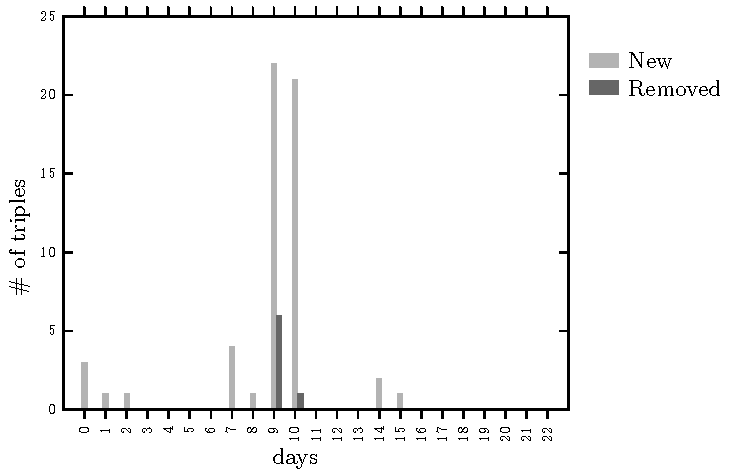
\includegraphics[width=0.8\textwidth]{images/updating_1.pdf}
  \end{center}
  \caption{Number of new upcoming movies, which are published on IMDb per day. Most movies are published between Thursdays to Sundays.}
  \label{fig_coming_soon_movie}
\end{figure}

This observation lead to the decision to update upcoming movies from IMDb on a daily basis.
TMDb and OFDb show similar results, so that upcoming movies from these data sources are updated daily, too.
The sandbox of Freebase, which is requested over the API, updates once a week.
This is why the upcoming movies from Freebase are only updated every week.

\subsubsection{Updating existing Movies}
In Figure \ref{fig_new_movie} the number of changed triples of a newly released movie from IMDb is displayed.
Therefor, a movie was crawled and triplified daily.
Obviously, the movie frequently changes in the first days.
Also, the number of changing triples decreases with time.
Triples changing often are mostly cast triples, links to images and videos, IMDb rating, character triples or taglines.

\begin{figure}[h!]
  \begin{center}
  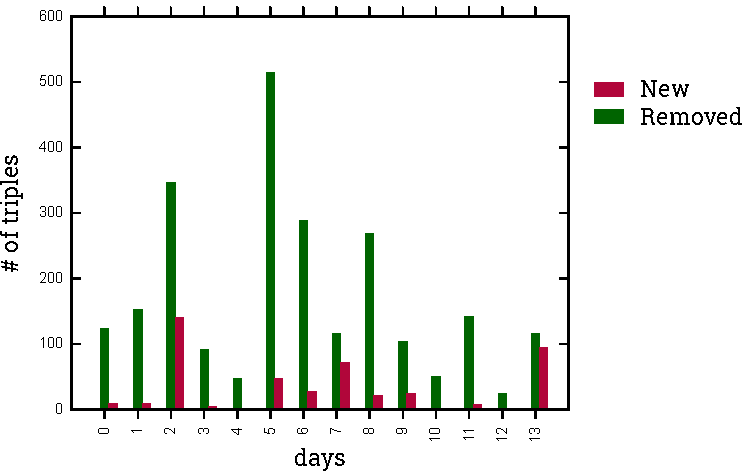
\includegraphics[width=0.8\textwidth]{images/updating_2.pdf}
  \end{center}
  \caption{Number of triples, which change in the first days of a newly released movie from IMDb. The older the movie gets, the less triples change.}
  \label{fig_new_movie}
\end{figure}

Because a movie changes less the older it is, existing movies are divided into different categories.
Each category is updated at different frequencies (Table \ref{tab_updating_existing}).
\begin{table}[ht]
	\begin{center}
	\begin{tabular}{rl}
		\textbf{Category of movie} & \textbf{Frequency} \\ \hline
		one year old & weekly \\
		5 year old & monthly \\
		5 - 25 years old & yearly \\
		older than 25 years & never \\
	\end{tabular}
	\end{center}
	\caption{Frequency of updating the different categories of existing movies.}
	\label{tab_updating_existing}
\end{table}
If a category should be updated, the scheduler does the following steps:
\begin{enumerate}
	\item Find all movies which should be updated regardless their original data source.
	\item For each of these movies, get the updated movie resource and triplify it.
	\item Delete all triples of the movie in the triple store in the corresponding graph.
	\item Load the new triples into the corresponding graph in the triple store.
\end{enumerate}
Because the movies are stored in different graphs depending on their original data source, the scheduler knows where to find the movie resource in the web.
The original resource of a movie is stored in a \emph{sameAs} triple.
Deleting the existing triples and storing the newly downloaded triples ensures that no conflicting information of a resource is stored.